\documentclass[a4paper,12pt]{article} % тип документа

% report, book

% Рисунки
\usepackage{graphicx}
\usepackage{wrapfig}

\usepackage{hyperref}
\usepackage[rgb]{xcolor}
\hypersetup{				% Гиперссылки
    colorlinks=true,       	% false: ссылки в рамках
	urlcolor=blue          % на URL
}

%  Русский язык

\usepackage[T2A]{fontenc}			% кодировка
\usepackage[utf8]{inputenc}			% кодировка исходного текста
\usepackage[english,russian]{babel}	% локализация и переносы


% Математика
\usepackage{amsmath,amsfonts,amssymb,amsthm,mathtools} 


\usepackage{wasysym}

\author{Анна Назарчук Б02-109}
\title{1.2.2 Экспериментальная проверка закона вращательного движения на крестообразном маятнике}
\date{}
\begin{document}
\maketitle

\section{Теоретические сведения}
Закон вращательного движения:
\begin{equation}
I\ddot{\varphi} = M
\end{equation}
$\ddot{\varphi} \equiv \dot{\omega} \equiv \beta$

\begin{figure}[h!]
\begin{center}
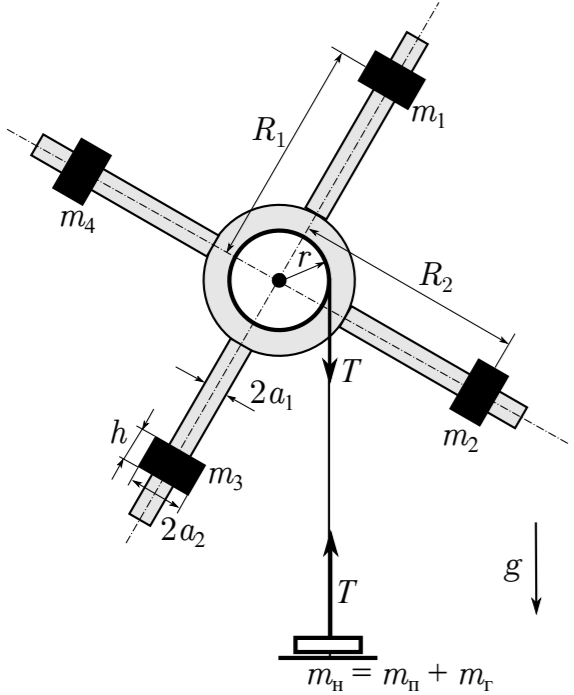
\includegraphics[width=0.5\textwidth]{Маятник}
\end{center}
\caption{Крестообразный маятник Обербека} \label{маятник}
\end{figure}
На маятник действуют два момента сил: силы натяжения нити ($M_T$) и трения ($M_\text{тр}$): $M_T = rT$, $r$ - радиус шкива. Для движения платформы с учетом нерастяжимости нити:
\[m_H \beta r = m_H\ddot{y} = m_Hg - T\]
Откуда согласно основному уравнению вращательного движения:
\begin{equation}
(I+m_Hr^2)\beta = m_Hgr-M_\text{тр}
\label{M_T}
\end{equation}

Рассмотрим момент силы трения. Его зависимость от скорости не ясна, однако может иметь как составляющую, пропорциональную силе реакции в оси $N$ (сухое трение), так и составляющую, пропорциональную угловой скорости вращения (вязкое трение). Откуда:
\begin{equation}
M_\text{тр} \simeq (1 + \frac{m_H}{m_M}) M_0 + \eta \omega \approx M_0 +\eta \omega
\label{трение}
\end{equation} 
где $M_0$ - момент сил трения для покоящегося маятника при нулевой массе подвеса, $m_M$ - масса маятника 

Для расчета момента инерции системы, предположим, что грузы $m_i$ имеют форму полых цилиндров, внутренний и внешний радиус которых известен, образующая h
\begin{equation}
I = I_0 + \sum_{i=1}^4(I_i+m_iR_i^2)
\label{I}
\end{equation}
где $I_0$ - момент инерции системы без грузов, $R_i$ -  расстояние от центров масс грузов до оси вращения
\begin{equation}
I_i = \frac{1}{12}m_ih^2+\frac{1}{4}m_i(a_1^2+a_2^2)
\label{Ii}
\end{equation} - момент инерции груза относительно оси, проходящей через его центр масс
\section{Экспериментальная установка}
В работе используется крестообразный маятник (рис. \ref{маятник}), состоит из четырех тонкий стержней, перпендикулярных друг другу, укрепленных на втулке. Втулка и два шкива насажены на общую ось, вся система благодаря подшипникам может вращаться вокруг горизонтальной оси. Установка позволяет автоматически фиксировать моменты прохождения концов стержня через датчик.

\section{Измерения и обработка данных}
\subsection{Балансировка}
Балансировка системы при помощи добаления грузов на стержни, при движении несбалансированного маятника слышны стуки в подшипниках, график зависимости ускорения от угловой скорости имеет пульсации (рис. \ref{пульсации})
\begin{figure}[h!]
\begin{center}
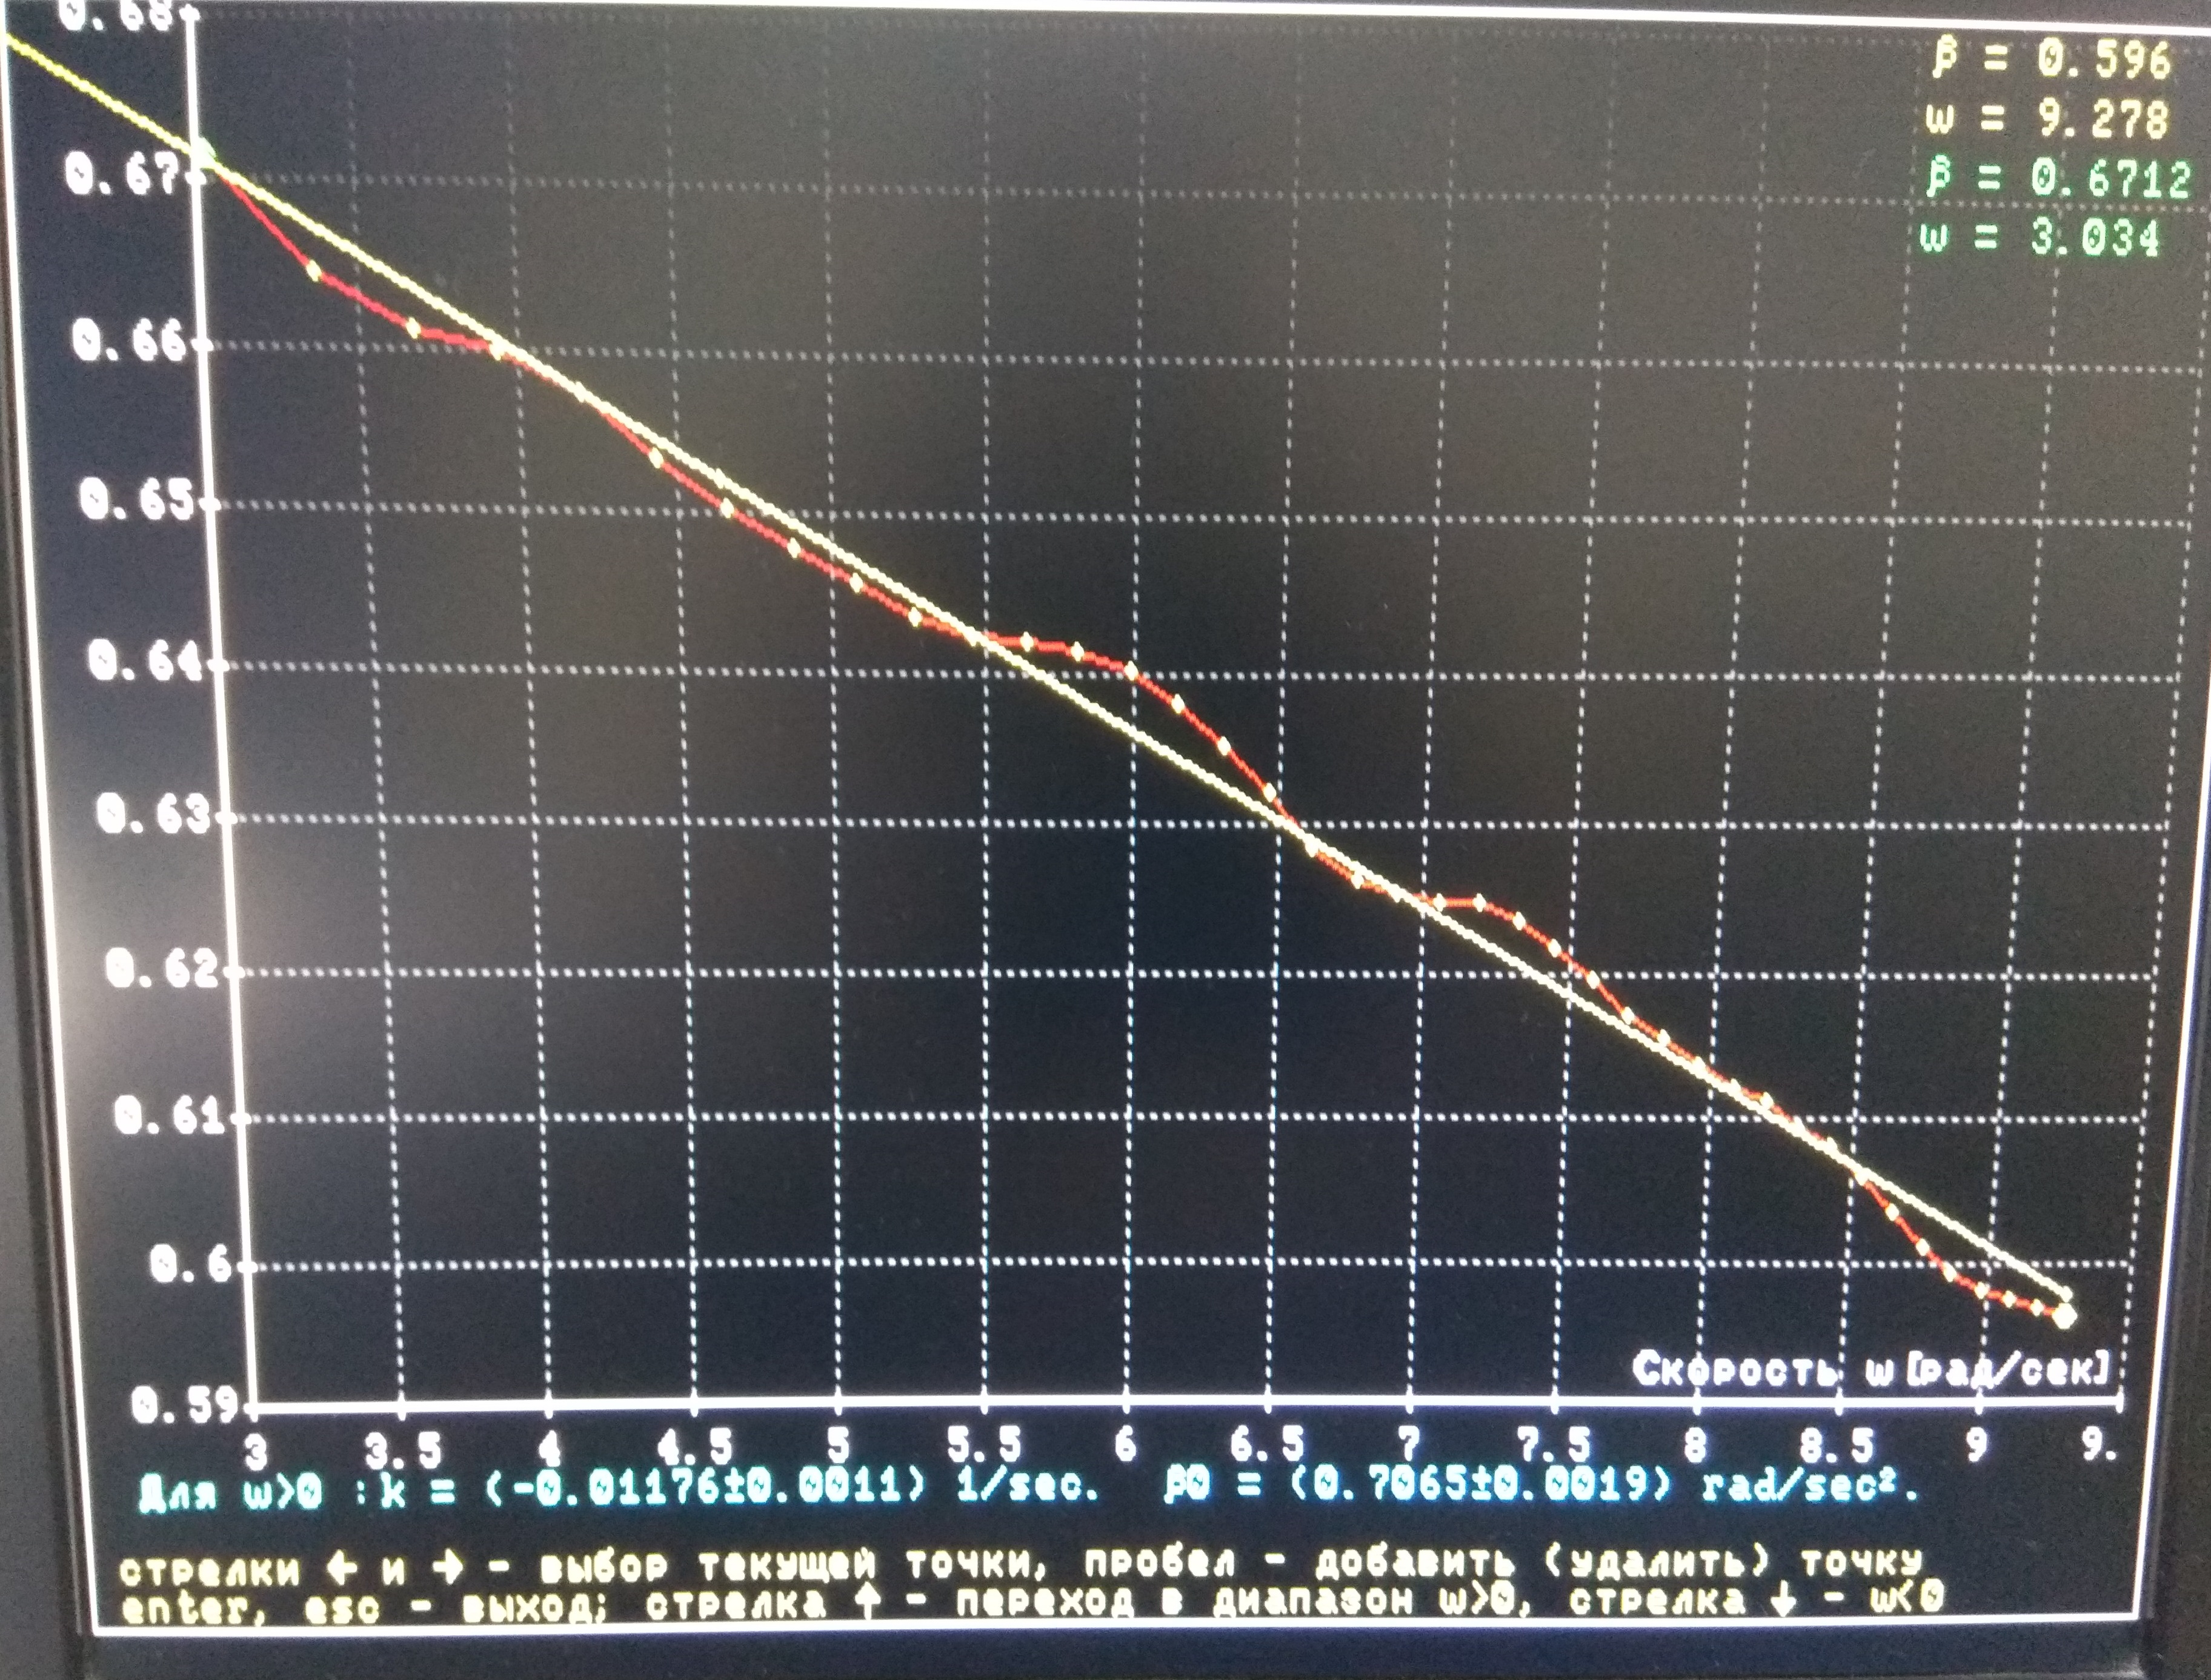
\includegraphics[width=0.7\textwidth]{Пульсации}
\end{center}
\caption{Пульсации при движении недостаточно сбалансированного маятника} \label{пульсации}
\end{figure}

\begin{table}
\caption{Характеристики системы в сбалансированном состоянии}
\begin{tabular}{|c|c|c|}
\hline 
№ груза & m, г & R, см \\ 
\hline 
1 & $155.5\pm 0.1$ & $8.2\pm 0.05$ \\ 
\hline 
2 & $148.9\pm 0.1$ & $8.6\pm 0.05$ \\ 
\hline 
3 & $151.9\pm 0.1$ & $9.4\pm 0.05$ \\ 
\hline 
4 & $150.1\pm 0.1$ & $9.5\pm 0.05$ \\ 
\hline 
\end{tabular} 
\end{table}
Маятник приходит в движение без добавления перегрузков, поэтому так момент силы трения в подшипниках измерить невозможно. Но можно сделать вывод, что:
\begin{equation}
M_0 < m_\text{п}gr = 2.9 \cdot 10^{-3}
\end{equation}

\subsection{Измерения с постоянным моментом инерции и разными перегрузками}

\begin{table}
\caption{Измерения с постоянным моментом инерции и разными перегрузками}
\label{Iconst}
\begin{tabular}{|c|c|c|c|c|c|c|c|c|c|}
\hline 
$m_\text{п}$, г & k, 1/с & $\sigma_k$, 1/с & $\beta_0$, рад/$c^2$ & $\sigma_{\beta_0}$, рад/$c^2$ & $R_1$, см & $R_2$,см & $R_3$, см & $R_4$, см & $r$, см \\
\hline 
0 & -0.005163 & 0.0023 & 0.1837 & 0.0015 & 8.2 & 8.6 & 9.4 & 9.5 & 1.75  \\ 
\hline
6.21 & -0.00831 & 0.0028 & 0.2607 & 0.0024 & 8.2 & 8.6 & 9.4 & 9.5 & 1.75 \\ 
\hline
9.07 & -0.0084 & 0.0018 & 0.3008 & 0.0016 & 8.2 & 8.6 & 9.4 & 9.5 & 1.75 \\ 
\hline
45 & -0.009674 & 0.002 & 0.7118 & 0.0027 & 8.2 & 8.6 & 9.4 & 9.5 & 1.75  \\ 
\hline
62 & -0.01475 & 0.0012 & 0.95 & 0.002 & 8.2 & 8.6 & 9.4 & 9.5 & 1.75  \\ 
\hline
51.5 & -0.01102 & 0.0055 & 0.7811 & 0.0074 & 8.2 & 8.6 & 9.4 & 9.5 & 1.75  \\ 
\hline
100 & -0.01176 & 0.0011 & 0.7065 & 0.0019 & 8.2 & 8.6 & 9.4 & 9.5 & 0.9  \\ 
\hline
103.55 & -0.01237 & 0.0013 & 0.7288 & 0.0023 & 8.2 & 8.6 & 9.4 & 9.5 & 0.9 \\ 
\hline
8.95 & -0.006902 & 0.0022 & 0.136 & 0.002 & 8.2 & 8.6 & 9.4 & 9.5 & 0.9  \\ 
\hline
64.2 & -0.00763 & 0.0027 & 0.4785 & 0.0029 & 8.2 & 8.6 & 9.4 & 9.5 & 0.9 \\ 
\hline
106 & -0.01022 & 0.0017 & 0.7382 & 0.0026 & 8.2 & 8.6 & 9.4 & 9.5 & 0.9 \\ 
\hline
\end{tabular} 
\end{table}
Значение k мало, можно считать, что угловое ускорение постоянно. По полученным данным (таблица \ref{Iconst}) и формуле \ref{M_T} построим график зависимости $\beta_0$ от $M_T$ (рис. \ref{betaM})


\begin{figure}[h!]
\begin{center}
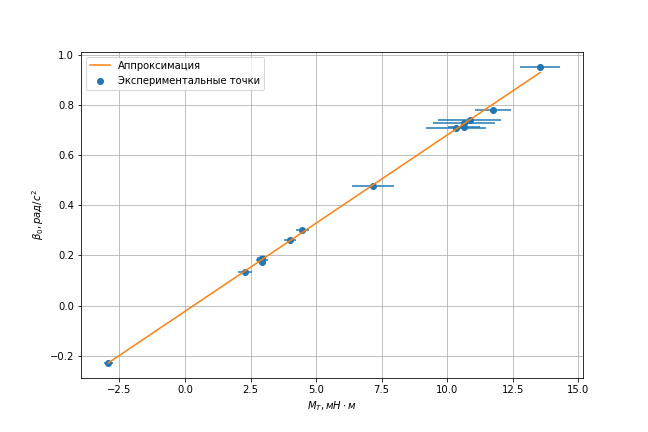
\includegraphics[width=\textwidth]{beta(M)}
\end{center}
\caption{Зависимость углового ускорения от момента силы натяжения нити} \label{betaM}
\end{figure}

Данные образуют прямую, что подтверждает справедливость уравнения вращательного движения. С помощью графика определим $M_0$ - момент сил трения для покоящегося маятника при нулевой массе подвеса и $I$ - момент инерции системы: $M_0 = 0.32 \pm 0.03 $ мН$\cdot$м, $I = 14.2 \pm 0.1$ г$\cdot \text{м}^2$

Получили, что $M_0 < m_\text{п}gr=2.93 \cdot 10^{-3}$, что согласуется с результами из предыдущих пунктов.

\subsection{Измерения с одинаковой массой перегрузка, но разными моментами инерции}

\begin{table}
\caption{Измерения с одинаковой массой перегрузка, но разными моментами инерции}
\label{mconst}
\begin{tabular}{|c|c|c|c|c|c|c|c|c|c|}
\hline 
$m_\text{п}$, г & k, 1/с & $\sigma_k$, 1/с & $\beta_0$, рад/$c^2$ & $\sigma_{\beta_0}$, рад/$c^2$ & $R_1$, см & $R_2$,см & $R_3$, см & $R_4$, см & $r$, см \\
\hline
100 & -0.002031 & 0.0037 & 1.587 & 0.0072 & 7.2 & 7.8 & 7.8 & 8.3 & 1.75\\
\hline
100 & -0.01096 & 0.0026 & 1.026 & 0.0036 & 11.9 & 11.6 & 12 & 12 & 1.75\\
\hline
100 & -0.0339 &  0.0024 & 2.501 & 0.0053 & 3.1 & 3.3 & 2.4 & 2.6 & 1.75\\
\hline
100 & -0.02494 & 0.0049 & 2.081 & 0.0085 & 4.6 & 5.6 & 4.6 & 4.7 & 1.75\\
\hline
100 & -0.02627 & 0.0098 & -2.013 & 0.018 & 4.6 & 5.6 & 4.6 & 4.7 & 1.75\\
\hline
100 & -0.01335 & 0.0041 & 0.8113 & 0.0066 & 7.2 & 7.8 & 7.8 & 8.3 & 0.9\\
\hline
100 & -0.003478 & 0.0099 & 0.504 & 0.013 & 11.9 & 11.6 & 12 & 12 & 0.9\\
\hline
100 & -0.02933 & 0.0035 & 1.294 & 0.0071 & 3.1 & 3.3 & 2.4 & 2.6 & 0.9\\
\hline
100 & -0.01663 & 0.0051 & 1.071 & 0.001 & 4.6 & 5.6 & 4.6 & 4.7 & 0.9\\
\hline

\end{tabular} 
\end{table}
Значение k мало, можно считать, что угловое ускорение постоянно. По полученным данным (таблица \ref{mconst}) и формуле \ref{M_T} найдем момент инерции системы в зависимости от положений грузов и построим график зависимости I от $\sum_i m_iR_i^2$ (рис. \ref{Imr2})

\begin{figure}[h!]
\begin{center}
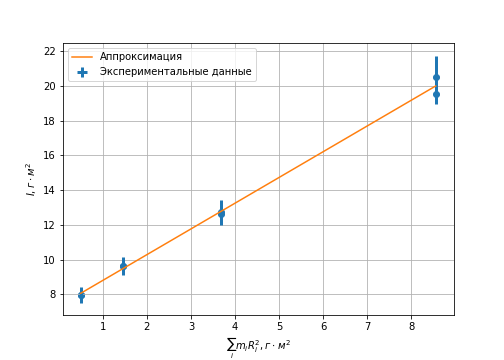
\includegraphics[width=\textwidth]{I(mr2)}
\end{center}
\caption{Зависимость момента инерции от положений грузов} \label{Imr2}
\end{figure}

Определим сумму $I_i$:
\[\sum_i I_i = \sum_i(\frac{1}{12}m_ih^2+\frac{1}{4}m_i(a_1^2+a_2^2)) = 7.3 \cdot 10^{-5} \text{ кг} \cdot \text{м}^2\]
Сумма значительно меньше сдвига (a) прямой графике, определенного по МНК, поэтому $I_0 \approx a$
С помощью графиков и формул (\ref{I} и \ref{Ii}) определим значение $I_0 = a = (73 \pm 0.91) \cdot 10^{-4} \text{ кг} \cdot \text{м}^2$

\subsection{Измерения без грузов}

\begin{table}
\caption{Измерения без грузов}
\label{mconst}
\begin{tabular}{|c|c|c|c|c|c|}
\hline 
$m_\text{п}$, г & k, 1/с & $\sigma_k$, 1/с & $\beta_0$, рад/$c^2$ & $\sigma_{\beta_0}$, рад/$c^2$ & $r$, см \\
\hline
100 & -0.0084  & 0.0018 & 2.87 & 0.0178 & 1.75\\
\hline
100 & -0.003478 & 0.0099 & 2.67 & 0.0211 & 1.75\\
\hline
100 & -0.006902 & 0.0022 & 1.41 & 0.0137 & 0.9\\
\hline
100 & -0.005464 & 0.002 & 1.76 & 0.0128 & 0.9\\
\hline
\end{tabular}
\end{table}
Из полученных данных можно определить $I_0 = (68 \pm 0.136) \cdot 10^{-4} \text{ кг} \cdot \text{м}^2$, что согласуется с результатами измерений предыдущим способом.

\subsection{Измерение коэффициента, отвечающего за вязкое трение}
Согласно формулам \ref{трение} и \ref{M_T} можно считать, что:
\begin{equation}
\eta = -m_\text{H}r^2k
\end{equation}
где k - коэффициент зависимости углового ускорения от угловой скорости. Из данных в таблице \ref{Iconst} получим, что:
\begin{table}
\caption{Коэффициент вязкого трения}
\begin{tabular}{|c|c|c|c|}
\hline 
масса перегрузка, г & k, 1/с & r, см & $\eta, $ $ 10^{-9}$ кг$\cdot$м$^2$/с\\
\hline
0 & -0.005163 & 1.75 & 2.695892719\\
\hline
6.21 & -0.00831 & 1.75 & 5.919524625\\
\hline
9.07 & -0.0084 & 1.75 & 6.71937\\
\hline
100 & -0.01176 & 0.9 & 11.1497148\\
\hline
103.55 & -0.01237 & 0.9 & 12.0837582\\
\hline
8.95 & -0.006902 & 0.9 & 1.4535612\\
\hline
64.2 & -0.00763 & 0.9 & 5.02149375\\
\hline
106 & -0.01022 & 0.9 & 10.1863251\\
\hline
\end{tabular} 
\end{table}

Исходя из полученных данных можно найти значение $\eta = (6.09 \pm 1.22) \cdot 10 ^{-9} $кг$\cdot$м$^2$/с. Однако из полученного значения можно сделать немного выводов ввиду высокой погрешности, но при данных скоростях можно пренебречь составляющей с вязким трением, так как значение существенно меньше момента сил трения для покоящегося маятника при нулевой массе подвеса, что подтверждает предполагаемые приближения.

\section{Вывод}
Экспериментально получена зависимость углового ускорения от момента прикладываемых к маятнику сил, тем самым подтверждено уравнение вращательного движения. Определен момент инерции маятника несколькими способами, приводящими к одному и тому же результату.
\end{document}